\documentclass[11pt]{article}
\usepackage[utf8]{inputenc}

\title{Generative Adversarial Networks}
\author{Jacob Smith}
\date{December 12, 2017}

\usepackage{natbib}
\usepackage{graphicx}
\usepackage[options ]{algorithm2e}
\usepackage{parskip}

\graphicspath{{./img/}}

\begin{document}
\maketitle

\begin{abstract}
    Deep generative networks have often fallen short, especial when compared to discriminative models. Since their conception in 2014, generative adversarial networks have seen exponential growth in research. These networks offer promising results for both unsupervised learning and generative models. This research paper presents an overview of generative adversarial networks. Specifically, we will examine the motivation behind GANs, their theoretical justification, the current state of GANs and the research frontiers that have yet to be explored.
\end{abstract}

\section{Introduction}
Deep learning have made astounding progress within the past decade. Discriminative models have recently surpassed the abilities of human within the domain of pattern recognition \citep{2014arXiv1404.7828S}. These successes can attributed to vast, high dimension datasets in conjunction with large neural networks using linear activation functions, dropout regularization techniques and backpropagation to update the parameters \citep{2014arXiv1406.2661G}. However, deep learning possesses many more ambitious goals. Until recently, success has mostly been seen with supervised classifiers; however, deep generative models now competitively rival their discriminative counterparts.

Generative models learn the joint probability distribution $p(x,y)$ of an input $x$ and label $y$ whereas discriminative models directly learn the conditional probability $p(y|x)$. Generative models may be used as classifiers using Bayes rules to calculate the conditional probability $p(x,y)$ which can then be used to make predictions \citep{NIPS2001_2020}. Depending on the model, knowledge of the probability distribution can be created both explicitly and implicitly \citep{Goodfellow-et-al-2016}. Those which do not directly model a probability distribution offer mechanisms which require implicit knowledge of the underlying distribution, such as creating a sample from that distribution \citep{Goodfellow-et-al-2016}. As humans, we are able to understand the world around us with tremendous precision. It is easy to underestimate the complexity of the data we process to accomplish this feat. Although progress within the machine learning field is rapidly advancing, computers still have limited understanding of the data the process. Generative models, especially deep generative models, offer promising results towards this goal \citep{genmodelingopenai}.

\begin{figure}
\centering
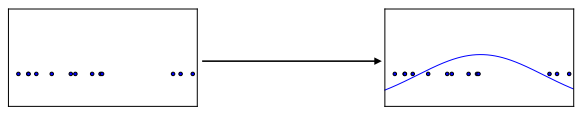
\includegraphics[scale=0.7]{pdf}
\caption{The process density estimation of one-dimensional data and a Gaussian distribution \citep{2017arXiv170100160G}. Generative models take a dataset $D$, sourced from a distribution $p_{data}$, a create an estimate of that distribution $p_{model}$.}
\label{fig:pdf}
\end{figure}

The process of training a generative model is very similar to a discriminative model. Using large amounts of data collected from a specific domain, we train the model to generate data from that domain. As these models have fewer parameters than that the number of data samples, they are forced to internalize some representation of the data. Although, unlike supervised training, there exists no explicit desired output. The problem becomes defining a cost function which forces the generative model to produce data more like that of the domain.

Generative adversarial networks (GANs), first introduced in 2014, offer a new framework for estimating generative models with use of an adversarial process \citep{2014arXiv1406.2661G}. These models offer a clever approach to solving the aforementioned problem of explicitly defining a cost function. Rather than training a single model, a discriminator is introduced. These two networks are pitted against each other in a minimax game. The generative model $G$ attempts to produce data that resembles that of the training set while the discriminative model $D$ attempts to classify whether or not a sample was real of generated. To train this network, $G$ attempts to maximize the error rate of $D$ whereas $D$ attempts to minimize it. Backpropagation is used to update the parameters and to train each model. In the ideal case, $D$ is unable to distinguish the generated samples from the real samples and produces an error rate of $\frac{1}{2}$ \citep{2014arXiv1406.2661G}.

\section{Motivations}
There exists several compelling reasons for studying generative modeling \citep{2017arXiv170100160G}. These models are extremely useful when your goal is understand the underlying distribution parameters. For example, joint probability distributions of high dimensional data is relevant to both applied math and engineering \citep{2017arXiv170100160G}. Generative models are also applicable to reinforcement learning, particularly model-based learning algorithms. A time series generative model, one which predicts future states of an environment given the current state of the environment and an agents actions, are of particular interest \citep{2017arXiv170100160G}. An agent may learn the best action to take in a given scenario by querying this generative model and choosing the one which outputs the best state of the world. Furthermore, generative models, especially GANs, have recently excelled at semi-supervised learning.

Proposed in the original GAN paper \citep{2014arXiv1406.2661G}, semi-supervised techniques used in conjunction with GANs have recently proven themselves as a reputable technique. The premise involves training the discriminator to classify images into $n + 1$ classes where $n$ is the number of class labels and the additional $1$ is the class of a fake image. This algorithm is able to obtain great performance on relatively small labeled datasets when compared to labeled datasets typically state of the art supervised algorithms \citep{2017arXiv170100160G}. Currently, the best performing semi-supervised GAN are feature matching GANs, where the new objective of the generative model is to minimize the distance between a layer $l$ of the discriminator \citep{2016arXiv160603498S}.

Many applications require multi-modal outputs. For example, predicting the next action of a self-driving car. Within this context, it is important the model not be trained by traditional methods, such as using mean squared error to minimize the distance between the expected and predicted actions. These models cannot be used in situations where there is more than one appropriate prediction. Generative modeling, especially GAN, allow machine learning to function the scenarios where one input corresponds to multiple acceptable outputs \citep{2017arXiv170100160G}.

Tasks which involve image generation, modification or translation are all highly applicable to generative models. Although GANs may be used to generate any type of data, images remain the most commonly used source of training data. Research conducted within the past three years demonstrates the capabilities of GANs to perform these tasks \citep{2017arXiv170100160G, 2016arXiv161102200T, 2014arXiv1411.1784M}. For example, GANs have recently been shown to be capable of translating aerial photographs into maps and sketches into realistic images \citep{2017arXiv170100160G}.

When compared to other generative models, especially deep generative models, GANs possess several advantages... quicker? no Markov chains?

\begin{figure}
\centering
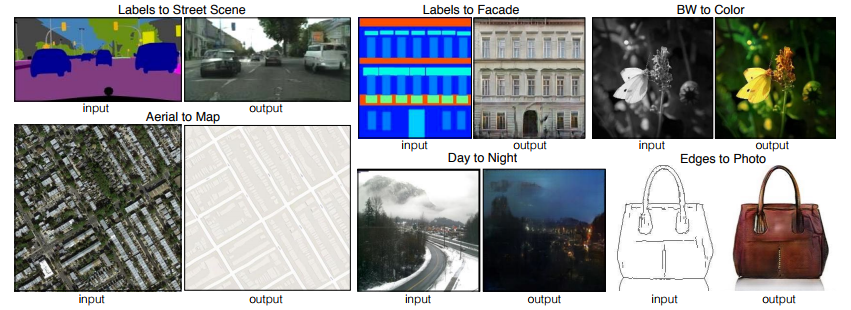
\includegraphics[scale=0.65]{img2img}
\caption{Examples of the image-to-image technique developed by Isola \textit{et al.} \citep{2016arXiv161107004I}. This approach makes use of conditional generative adversarial networks to map image domains.}
\label{fig:Image to Image Examples}
\end{figure}

\section{Background}
Generative adversarial networks may use any differentiable functions for the models; however, the optimal results are typically achieved when neural networks are used \citep{2014arXiv1406.2661G}. We first define a vector $z$ such that $z~p_z(z)$. This vector becomes the argument of the generator $G(z;\theta_g)$ where $G$ is a differentiable function and $\theta_g$ is its parameters. Another differentiable function $D(x;\theta_d)$ for the discriminator. This function takes as input a vector $x$, either from the output of $G$ or a sample from the training set, and is parametrized by $\theta_d$. The output of the discriminator is a scalar number representation the probability that the arguments were derived from the training data. In this situation, there exists a minimax game where $D$ attempts to maximize the probability of assigning a correct label and $G$ attempts to minimize $\log(1-D(G(z)))$. The networks $G$ and $D$ play a minimax game with the value function $V(D,G)$:

$$\min_{G}\max_{D}V(D, G) = \mathbb{E}_{x\sim p_{data}(x)}[\log(D(x))] + \mathbb{E}_{z\sim p_z(z)}[\log(1-D(G(z)))]$$

For the training step, any variant of gradient descent may be used with respect to the individual cost functions \citep{2017arXiv170100160G}. The first updates $\theta_D$ while attempting to minimize the discriminator cost function $J_D$ while the other updates $\theta_G$ while attempting to minimize the generator cost function $J_G$. There exist several variations of the cost function that may be used for training purposes; however, the discriminator cost has remained the same for each.

$$J_d(\theta_D,\theta\G) = -\frac{1}{2}\mathbb{E}_{x\sim p_{data}(x)}[\log(D(x))] - \frac{1}{2}\mathbb{E}_{z\sim p_{z}(z)}[\log(1-D(G(z)))]$$

This is a standard cross entropy cost function that is trained on two minibatches, one from the dataset and one from the generator. For this to become a zero-sum game, a minimax game, the cost function of the generator is simply the negation of the discriminator.

$$J_g(\theta_D,\theta\G) = -J_d(\theta_D,\theta\G)$$

This version of the generator loss function is particularly useful for theoretical analysis as shown in the first GAN paper \citep{2014arXiv1406.2661G}. It can be shown that the minimax game is the same as minimizing the Jensen-Shannon divergence and that each player will eventually converge if both players are able to directly update the function space as oppose to the parameters within a neural network \citep{2017arXiv170100160G}. However, in this minimax version, the loss function of the generator suffers from a vanishing gradient when the discriminator confidently rejects the generated data. The solution proposed by Goodfellow is to train the generator to maximize $log(D(G(z)))$ rather than minimize $log(1-D(G(z)))$ \citep{2014arXiv1406.2661G}. This function is heuristically motivated as to provide strong gradients when either the generator or discriminator is not functioning optimally.

$$J_g(\theta_D,\theta\G) = -\frac{1}{2}\mathbb{E}_{z\sim p_{z}(z)}[\log(D(G(z)))]$$



\begin{algorithm}[H]
  \SetAlgoLined
  \Input{$n$: The number of training iterations} \linebreak
  \Input{$k$: The number of discriminator iterations} \linebreak
  \For{training iteration in n} {
    \For{discriminator iteration in k} {
      sample $m$ vectors $\{z^{(1)},...,z^{(m)}\}$ from distribution $p_z(z)$\;
      sample $m$ vectors $\{x^{(1)},...,x^{(m)}\}$ from the training samples\;
      update the discriminator using its stochastic gradient
      $$\nabla_{\theta_d}\frac{1}{m}\sum_{i=1}^{m}[\log(D(x^{(i)}))+\log(1-D(G(z^{(i)})))]$$
    }
    sample $m$ vectors $\{z^{(1)},...,z^{(m)}\}$ from distribution $p_z(z)$\;
    update the generator using its stochastic gradient\;
    $$\nabla_{\theta_g}\frac{1}{m}\sum_{i=1}^{m}[\log(1-D(G(z^{(i)})))]$$
  }
  \caption{The initial generative adversarial network algorithm developed by Goodfellow \textit{et al.} in 2014 \citep{2014arXiv1406.2661G}. Multiple variations of this algorithm have since been produced. One of the benefits of adversarial networks is that they may be updated using regular gradient descent.}
\end{algorithm}

This algorithm presents the initial training algorithm used by Goodfellow \textit{et al.} when GANs were introduced in 2014 \citep{2014arXiv1406.2661G}. Many modifications have been made by various sources. The first step in the algorithm is to optimize the discriminator $D$. Optimally, one would train $D$ to completion; however, this is unrealistic in practice. The number of discriminator training iterations becomes a hyperparameter of the algorithm. For the initial GAN experiments, this number was set to $1$ to reduce computation time. The preferable value for this hyperparameter is still largely debated amongst researchers \citep{2017arXiv170100160G}.

\section{Issues}
Generative adversarial networks are often characterized by their instability. The training process of

Shape, count, orientation

\section{Improvements}
Feature matching



\section{Model Variations}
Deep Convolutional GAN

Wasserstein GAN to improve stability

Reccurent GAN

Conditinal GAN

Growing GANs

\section{Research Frontiers}
GANs are an exciting idea that are currently leading the frontier of deep generative models.

Hiton's Capsule Network

Improving the stability of GANs

\section{Conclusion}
Generative models are currently being applied to many problems \citep{genmodelingopenai}; however, they offer many more possibilities due to their ability to understand the data they are given.

\bibliographystyle{plain}
\bibliography{references}
\end{document}
